\documentclass[conference]{IEEEtran}
%\IEEEoverridecommandlockouts
% The preceding line is only needed to identify funding in the first footnote. If that is unneeded, please comment it out.
\usepackage{cite}
\usepackage{amsmath,amssymb,amsfonts}
\usepackage{algorithmic}
\usepackage{graphicx}
\usepackage{float}
\usepackage{subfig}
\usepackage{textcomp}
\usepackage{xcolor}
\usepackage[british]{babel}
\newcommand\T{\rule{0pt}{2.6ex}}       % Top strut
\newcommand\B{\rule[-1.2ex]{0pt}{0pt}} % Bottom strut
\def\BibTeX{{\rm B\kern-.05em{\sc i\kern-.025em b}\kern-.08em
        T\kern-.1667em\lower.7ex\hbox{E}\kern-.125emX}}
\begin{document}

\title{FPGA Based Modelling of an ADPLL Network\\}

\author{\IEEEauthorblockN{C. Dooley, E. Blokhina, B. Mulkeen}
    \IEEEauthorblockA{\textit{School of Electrical \& Electronic Engineering, University College Dublin}
    	\vspace{-1.2cm}
	}
}
\maketitle
\begin{abstract}
    This paper introduces and compares the implementation of a number of FPGA based ADPLL network prototyping architectures. Comparison is then made between the expected performance and role of each method as a development tool.
\end{abstract}
\section{Motivation}
The technical motivation underlying this paper is the creation of an Field Programmable Gate Array (FPGA) based prototyping platform for All Digital Phase Lock Loop (ADPLL) networks. As the creation of Application Specific Integrated Circuits (ASICs) is an expensive and time consuming process, and mistakes made in the design may require the manufacture of a new chip, it is important to ensure that any errors made in the design have been located and addressed before manufacture..
Simulations either at theoretical or gate/transistor levels have global usage in minimising such errors due to the ubiquity of simulators and their ease of use.\\
However simulations are only as good as the model used to describe the dynamics of the system, and emulating real jitter and other behaviours of a complex system is a rather difficult task. %TODO wording of this last sentence
An FPGA based prototype allows the system designers to validate the performance of both design and simulation, particularly the response to key noise sources such as power supply noise. An FPGA is ideal for this task as it leverages the existing skill set of a digital designer, permits the re-use of certain blocks, and most importantly enables cost effective and rapid reworking of the design.\\
An FPGA as a prototyping tool has seen use in UPMC Sorbonne and University College Dublin, and has been used in the testing of established designs prior to their implementation in custom silicon \cite{zianbetov2013phd,shan2014phd}, the validation of realistic models for use in high level simulations\cite{theboys2019} and the exploration of new designs for digital blocks before progressing on to true digital design on a gate level.  %TODO references
In the case of Shan et. al \cite{shan2014phd}, direct testing of control parameters was performed using an FPGA based design, where all parameters were scaled down proportionally and thus the ideal gains for the loop filter found in simulation, could be tested in a more realistic setting.\\
Similarly Koskin et. al \cite{theboys2019} used the analysis of a number of ADPLLs implemented on an FPGA, both independently and in a network, to validate previously obtained theoretical results while avoiding the costs associated with the development of a custom IC.\\
Prototyping on an FPGA does have its drawbacks, most notably the mixed-signal circuits central to the operation of an ADPLL are not implementable on an FPGA and while most fundamental digital circuit elements are present these elements are not true transistor level implementations of their functionality but rather implemented by lookup tables and other multi-role structures on the FPGA. These drawbacks present a challenge to a designer as they restrict the potential architecture of key blocks. This is of particular concern when trying to mimic the behaviour of an established design on an FPGA.\\
The particular system that this paper will discuss is an ADPLL network. This is based on an idea first proposed in a 1995 paper by Pratt and Nguyen \cite{pratt1995distributed}, in which they proposed an alternative clock distribution network for ICs using a Cartesian grid of clocking areas, each with their own Phase Lock Loop, which has become known as a PLL Network . This methodology was implemented by Gutnik et. al \cite{gutnik2000active} who found it to be feasible. Subsequently Javiden et. al
\cite{javidan2011all} proposed the implementation of such a system using All Digital PLLs, which better suited the use cases of the technology and avoided some of the flaws pointed out in the original paper. Zianbetov and Shan followed on from this proposition by implementing such a network on a custom IC \cite{zianbetov2013phd,shan2014phd}.\\
This paper will examine the process of creating such a system, highlight the differences between potential designs and address some of the challenges and pitfalls that may be encountered along the way. This paper will also demonstrate that FPGA based prototyping can play a central role on the pathway to the implementation of an ADPLL network on a custom chip, or indeed any number of similar applications. The paper is organised as follows: Section II describes the system that will be used on the FPGA and Section III the implementation thereof and the challenges encountered in the process. Finally, Section IV will present example measurements made on the platform and discuss their merit.

\section{System Architecture}
An ADPLL network, as the name would suggest, is created from a number of ADPLLs that are coupled using digital phase comparators which attempt to measure the phase error between two oscillators, with each non edge node being connected to four neighbours. Figure \ref{fig:adpll_network} illustrates such a system on a small scale, with a number of ADPLLs laid out in a Cartesian grid. The individual ADPLLs, often called distributed ADPLLs as the phase detectors are shared between nodes, are made up of a digitally controllable oscillator, an error combination block and a digital loop filter with the aforementioned digital phase detectors lying between each pair of oscillators.
\begin{figure}[h]
    \centering
    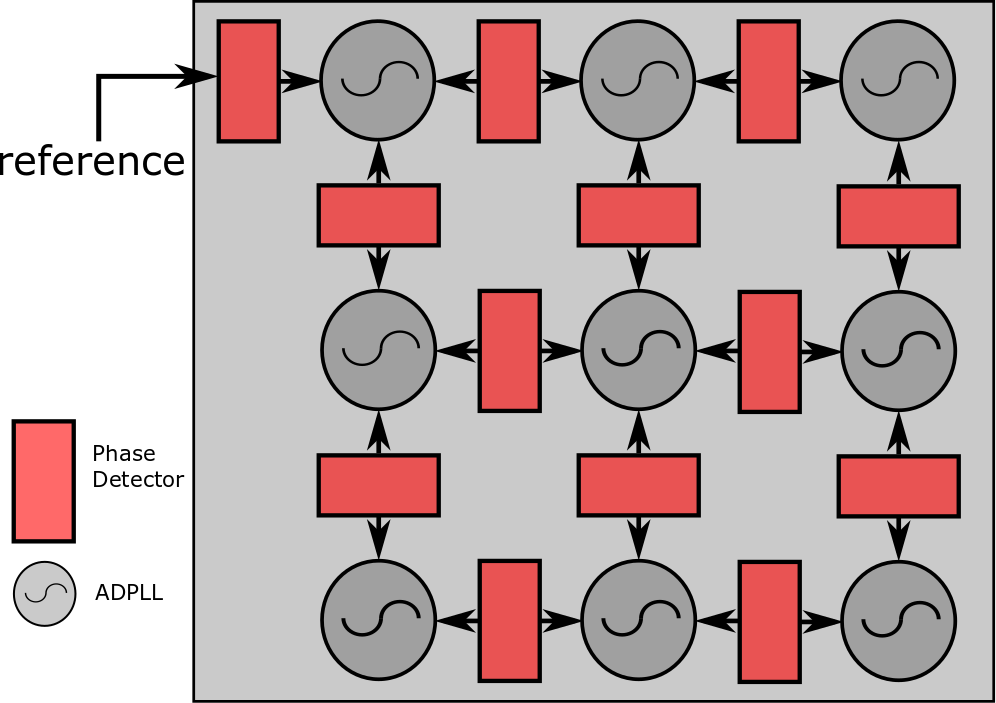
\includegraphics[width=0.25\textwidth]{adpll_network}
    \caption{ADPLL Network Architecture.}
    \label{fig:adpll_network}
    \vspace{0.5cm}
    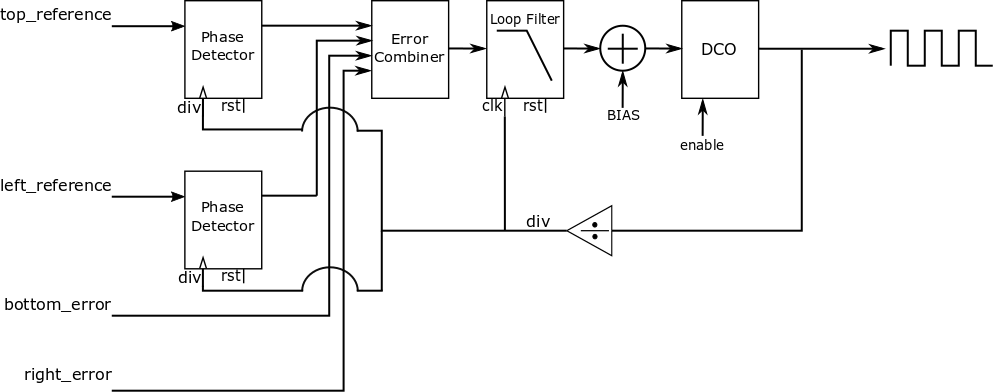
\includegraphics[width=0.4\textwidth]{dist_adpll}
    \caption{Distributed ADPLL Design.}
    \label{fig:adpll_base}
    \vspace{-0.5cm}
\end{figure}
\subsection{Digitally Controlled Oscillators}
While regular Voltage Controlled Oscillator (VCO) is tuned by the input voltage over a continuous range of values, in a digital system there are a very limited number of voltages representable, most commonly just two levels. As such, using the voltage itself to control an oscillator is not a viable strategy and instead Digitally (or Numerically) Controlled Oscillators (DCO) accept an \textit{n} bit wide control signal that alters the period of the output waveform. While tuning range, centre frequency and linearity apply as in a VCO, a DCO also has a minimum frequency step as a result of the non continuous control values. %TODO WORDING
In combination with the bit width of the control signal, the minimum frequency step limits the range over which the oscillator can be tuned. Frequently the output of the DCO is divided down to allow the control blocks in the feedback path that are clocked on this signal, to run at a lower and thus easier frequency.
\subsection{Loop Filter}
The loop filter is a key aspect of a phase lock loop as without it only the current output of the phase detector could be used to compute the control voltage of the VCO.
In an ADPLL it performs an identical role however, the digital environment results in the traditional loop filter being replaced by a discrete time Proportional Integral (PI) controller, with the integral path of the controller implemented by an accumulator.
\subsection{Error Combiner}
The Error Combiner, as the name suggests, performs a summation of the error signals from the phase detectors lying between any neighbouring oscillator and its neighbours. It is often convenient for this to be performed as a weighted sum, thus avoiding different gain requirements for the loop filter of oscillators in the corners of the grid that only have a pair of neighbours. The ability to change the weights during operation enables ``uni-directional start-up'', which Javiden et. al \cite{javidan2011all} found prevented the system from entering unwanted stable equilibriums warned of in Pratt and Nguyen's seminal paper.
\subsection{Phase Detector}
In a conventional PLL the phase detector measures a value proportional to the difference in phase between a pair of signals, which is then output as a continuous voltage.
A digital phase detector then attempts to do the same by measuring the time difference between fixed reference points in the waveform, which as a digital system deals with square waves, is typically the rising edge of each input to the block.
As in the oscillator, quantisation also plays a role in the behaviour of this block, with the time difference between each rising edge having a minimum possible measurement step.
In distributed ADPLLs the phase detector has dual outputs, each the inverse of the other, in order to feed the correct value to both of the connected error combiners. 

\section{FPGA Prototyping}
\subsection{FPGA Restrictions}
The use of an FPGA comes with many restrictions as to how a complex system such as an ADPLL can be designed with the mixed signal blocks, the DCO and phase detectors in particular being curtailed by the lack of transistor level control of the design and layout.\\
Two potential solutions exist which alleviate this problem, and are suited to different frequency ranges and/or goals of the designer. Firstly the clock signal generated by the FPGA's clock distribution block can be used to drive accumulator based oscillators and phase detectors, a technique suitable in two main use cases: The emulation of the performance of an already designed system operating at a proportionally cut down frequency or if the target frequency is low. 
The downside of this approach is that the minimum steps are dictated by the clock frequency of the FPGA, which at frequencies that are not orders of magnitude lower than the FPGA clock will result in coarse resolutions for detector or oscillator, and thus greater jitter seen at the oscillator output.
Accordingly this method only suitable for use at frequencies that are orders of magnitude lower than the maximum obtainable clock frequency of the FPGA's clock manager.\\
The second solution to the problem is more akin to the real world system, and uses the delay through primitive elements such as inverters, which can be deduced from measurements on the FPGA of choice but will vary depending on the layout selected. In the case of the FPGA used for this paper, a Xilinx Artix-7 (XC7A100T-1CSG324C), this delay is in the region of 300 picoseconds but varies depending on the routing between elements. This design is better suited to scenarios where the desired operating frequency is a significant fraction of the maximum usable clock of the FPGA or it is particularly desirable to have asynchronous behaviour in the system as in an ASIC. It is not suited to lower frequency designs as the number of inverters required will run into spacial constraints.
\subsection{Digitally Controlled Oscillators on an FPGA}
There are three key designs that be used to implement a DCO on an FPGA, two relying on the FPGA clock and one using inverter primitives. Each of these designs fulfils a different role in mimicking the behaviour of an ASIC based mixed signal DCO.

%\subsubsection*{Design 1}
%The first of these is a linear in period design using an accumulator architecture, with a variable reload value on overflow. Here the control code modifies the reload value around a bias point and thus adjusts the time taken for overflow to be reached with the oscillator's period given as $T_{osc} = (2^{\textrm{width}} - (\textrm{bias}+\textrm{code}))\times\textrm{clock period}$. Period linearity is a desirable characteristic as it mimics the behaviour of many mixed-signal implementations, and is the key use case of this method. The choice of the accumulator's Most Significant Bit (MSB) as the output signal however highlights the drawbacks of this method as less than half of the control codes are feasible. As the minimum period is set by the number of unused bits and the maximum period fixed at twice the minimum the frequency and tuning range combinations are very limited.
%In addition the wave output by this oscillator is only square at the maximum period and control code changes vary the duty cycle of the signal.

\subsubsection*{Design 1}
If frequency linearity is a desired characteristic of the oscillator, an accumulator based, FPGA clock driven design is possible. 
Here the control code $k$ is added to the value stored in the accumulator at each rising edge of the FPGA clock until overflow is reached at $2^n-1$, where $n$ is the bit width of the counter, thus valuing each control code increment at $\frac{\textrm{FPGA clock}}{2^{\textrm{width}}}$ Hz. The accumulator's Most Significant Bit (MSB) is used as the output of this block and forms a square wave.
This design is better suited to lower frequencies, where the output of the DCO is orders of magnitude lower than the clock signal driving it, as this ensures that the incremental change due to the control code remains a small fraction of the period.

\subsubsection*{Design 2}
The second potential DCO design is an inverter ring/chain which makes use of the delay through inverter primitives, thus bearing significant resemblance to DCOs used on ASICs. On an FPGA, the lack of precise control over the layout of blocks, means the exact value of the delay is uncertain and may vary noticeably from one implementation to another, however, this misalignment and the asynchronous behaviour stemming from the lack of an FPGA driven clock, increase the similarity between this design and an ASIC. The period is set by the number of inverters at $2\times(\textrm{num inverters})\times(\textrm{delay})$, and is varied by adding or removing a pair of inverters for every control code increment. This design works best when the desired period is within a couple orders of magnitude of the delay through each pair of inverters, beyond this point, the number of look-up tables and routing resources required to implement the design becomes unsustainable.\\
A third potential design exists, similar to Oscillator 1 in which the control code varies the reload value of the accumulator at overflow, however, this design will not be discussed in this paper.

\subsection{Phase Detectors on an FPGA}
The two options for replicating the behaviour of a phase detector also employ the same two design principles, with the option better suited to lower frequency signals once again, being driven by the clock generated by the FPGA and an inverter based design better suiting higher frequency systems, where the greater resolution offered is beneficial.\\
A  Sign-Number (SigNum) detector is a common method of performing phase-frequency detection in an ADPLL and is the method that will be discussed in this paper. As the name suggests, this design constitutes two sections, with one determining the sign of the phase difference and the other, its magnitude. The first issue with implementing a phase detector on an FPGA is the issue of metastability, where the output of a circuit element is at an undetermined level, which can occur if both signals were to have edges within a short time of one another or the set-up/hold times of a register are violated. This issue is easily addressed in an ASIC with an arbiter, however, an arbiter is a mixed signal circuit that is not synthesisable on an FPGA.

\subsubsection*{Design A}
The first potential design uses a Finite State Machine (FSM) to determine which edge has occurred first and thus the sign, and a counter that computes the time difference between each rising edge of each signal. This counter is clocked by the FPGA clock, thus giving the system a time resolution of $\frac{1}{F_{\textrm{FPGA}}}$. As with the FPGA driven oscillator, this results in a design that is only suitable when the frequency of operation is well below that of the FPGA clock due to resolution constraints. In order to avoid the problem of metastability, the incoming waveforms can be synchronised to the clock of the FPGA for no penalty beyond the extra clock cycle taken, as this synchronisation performs the same quantisation that would otherwise have occurred in the counter measuring the time difference. This design is better suited for use with the accumulator based oscillators due to the overlapping suitable frequency ranges, however, it can also be used in conjunction with an inverter ring. 
%Important to note is that in the case of the Artix-7 used in this paper, this results in a four times worse phase difference resolution than period resolution which made low jitter operation difficult, but this combination could be made possible by removing eight rather than two inverters for each control code step. %TODO plot this later

\subsubsection*{Design B}
Better suited for use with the inverter based oscillator, is a system that mimics the behaviour of a tapped delay line, working asynchronously to the FPGA clock. As the FPGA clock is not used, and that of the ADPLL cannot be used to measure itself, an unclocked sign detection circuit is required, an example of which can be seen in Figure \ref{fig:segn_pdetdl}. This is nearly identical to sign detection methods used on an ASIC, with the arbitration circuit replaced by a second SR Latch, which alleviates the issue of metastability.\\
A tapped delay line can be emulated on an FPGA through the use of inverter pairs, due to their short and approximately known delay placed between each tap.
The resolution then is the propagation time through the pair, although this will once again depend on the layout specifics, which was approximately 600 picoseconds on an Artix-7. This is significantly lower than the 4 nanoseconds achieved using the previous design and thus more suitable for use with an inverter ring oscillator, as this resolution is better than the time resolution of the oscillator. Figure \ref{fig:num_pdetdl} illustrates the configuration of the circuit used to emulate the function of a delay line that will be used in this paper.
\begin{figure}[h]
    \centering
    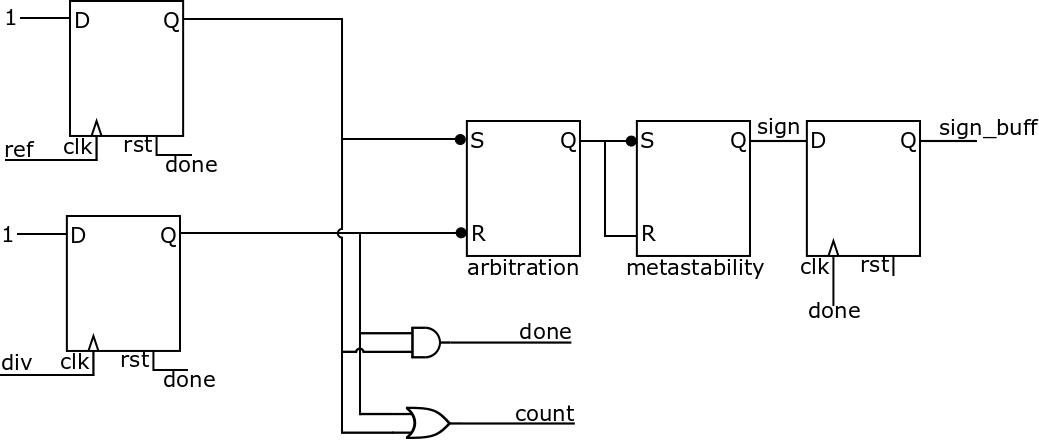
\includegraphics[width=0.4\textwidth]{../new_pdet1}
    \caption{Design B Sign Detection RTL Diagram.}
    \label{fig:segn_pdetdl}
    \vspace{-0.5cm}
\end{figure}
\begin{figure}[h]
    \centering
    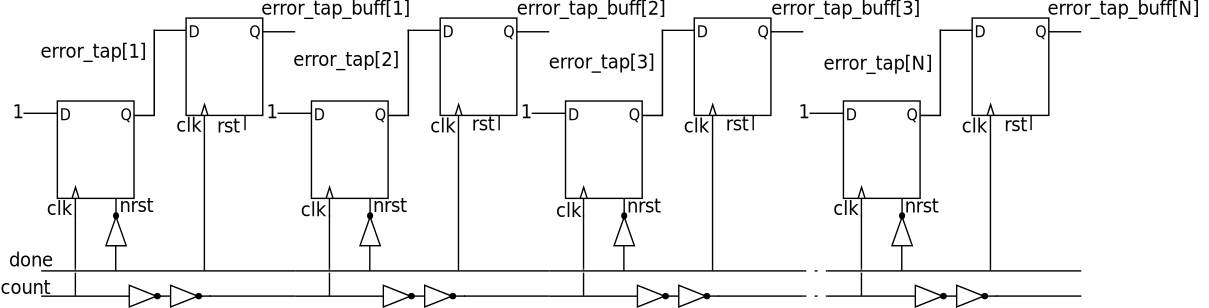
\includegraphics[width=0.4\textwidth]{../new_pdet2}
    \caption{Tapped Delay Line Emulation RTL Diagram.}
    \label{fig:num_pdetdl}
    \vspace{-0.5cm}
\end{figure}
\section{Comparison of Designs}
This paper will now examine the performance of a number of combinations of these blocks and the performance thereof, specifically oscillator 1 with phase detector A and oscillator 2 with detectors A \& B. For each test there were four ADPLLs on the FPGA arranged in a Cartesian Grid and as such each ADPLL will be referred to using matrix indexing corresponding to their grid location. For each configuration three different modes of operation were examined: Each ADPLL locked to the same 5 MHz external reference, each ADPLL connected to the left and above neighbours in a ``uni-directional'' network and finally a true ADPLL network where all neighbours are connected. For comparison, each configuration uses loop filter gains which had previously been determined to provide the best jitter performance. The data was captured using an Agilent MSO7054-A oscilloscope at 4 GSa/s. Each point of data is the mean of five 200 microsecond long captures which were then analysed in Matlab, Table \ref{table:b_c_perf} displays the results of this analysis.
The first columns of the table relate to the cycle-to-cycle jitter of the system, the difference between sequential rising edges, and the second portion gives the Time Interval Error, the difference between the actual timing of the edge and the ``ideal'' time as set by the reference. This combination of measurements will show how well each design performs the task of staying consistent from cycle to cycle both in relation to itself and the system at large.

\begin{table}[!ht]
    \begin{center}
        \begin{tiny}
        	\setlength{\tabcolsep}{.9\tabcolsep}
            \begin{tabular}{cc|c|c|c|c|c|c|}           
                \cline{3-8}
                && \multicolumn{3}{c|}{Jitter Standard Deviation (ns)} & \multicolumn{3}{c|}{Max. Time Interval Error. (ns)} \T\\
                \cline{3-8} 
                &&PLL 11&PLL 12&PLL 22&PLL 11&PLL 12&PLL 22\T\\
                \hline
                \multicolumn{2}{|l|}{Osc 1, PDET A}&-&-&-&-&-&-\T\\
                \multicolumn{2}{|r|}{Free PLLs} &1.4377 &1.4714&1.4217  &6.1910&6.3667&6.8052 \T\\
                \multicolumn{2}{|r|}{Uni-dir.}  &0.91589&1.0993&1.0875  &8.3619&8.9768&10.974 \T\\
                \multicolumn{2}{|r|}{Bi-dir.}   &1.0470 &1.0979&1.0306  &24.998&33.767&33.204 \T\\
                \hline
                \multicolumn{2}{|l|}{Osc 2, PDET A}&-&-&-&-&-&-\T\\
                \multicolumn{2}{|r|}{Free PLLs} &0.56728&0& 0&5.3797&0&0 \T\\
                \multicolumn{2}{|r|}{Uni-dir.}  &0.57365&0& 0&6.0632&0&0 \T\\
                \multicolumn{2}{|r|}{Bi-dir.}   &0.58760&0& 0&15.466&0&0 \T\\
                \hline
                \multicolumn{2}{|l|}{Osc 2, PDET B}&-&-&-&-&-&-\T\\
                \multicolumn{2}{|r|}{Free PLLs} &0.71635&0&0  &4.8293&0&0 \T\\
                \multicolumn{2}{|r|}{Uni-dir.}  &0.76883&0&0  &4.7922&0&0 \T\\
                \multicolumn{2}{|r|}{Bi-dir.}   &0.79292&0&0  &6.5277&0&0 \T\\
                \hline
                \B
                %% old 2b
                %&7.8090&7.8827&6.6272   &17.336&21.151&24.302
                %&7.7866&8.1145&7.3598   &17.649&29.962&37.051
                %&7.7575&7.7729&6.6962   &30.019&40.577&45.617
                %% old 2a
                %&78.458&74.025&67.779  &146.09&143.70&142.03
                %&78.428&72.646&65.665  &146.23&298.49&200.10
                %&78.436&73.827&67.648  &235.73&497.60&311.28
                
                %&5.6728e-10&0&0&5.3797e-09&0&0
                %&5.7365e-10&0&0&6.0632e-09&0&0
                %&5.8760e-10&0&0&1.5466e-08&0&0
                
            \end{tabular}
        \end{tiny}
        \caption{}
        \label{table:b_c_perf}
    \end{center}
\vspace{-0.5cm}
\end{table}
From the table it is apparent that the coarser period and detection steps of Design ``1A''  (3.875 nanoseconds as at greater clock frequencies timing violations would occur) cannot deliver the same jitter performance as the inverter ring driven designs. Looking at the two subsequent designs their lesser flexibility is made up for by their more realistic jitter behaviour. As would be expected best performance occurs when the network is in PLL mode and as the quality of the reference degrades as the network is connected up performance becomes worse. In terms of cycle-to-cycle jitter the best performing design is that of ``2A'', however, its time interval error is significantly worse especially in bilateral network mode. This more aggressive degradation as the network is linked up can be attributed to the worse detection resolution of the FPGA clocked phase detector, four times worse than the 1.2 second step of the entirely inverter based Design ``2B''.\\
The further a PLL is away from the reference feeding ADPLL 11 the worse performance is, peaking furthest from the reference in ADPLL 22.
%TODO insert comment here when I have more oscillators for 1 lines or so.

The lesser cycle-to-cycle of Design ``2A'' follows from the implementation independent design of the phase detector. Unlike the inverter based design where the implementation may result in the propagation delay between taps on the delay line changing, from both tap to tap in the same detector and the same tap in different detectors, the clocked design has identical detection resolutions as each register is driven by the FPGA clock. This can be highlighted in the more easily demonstrable case of the clocked and inverter based oscillators.\\
\begin{figure}[h]%
    \centering
    \subfloat[Inverter Based Design.]{{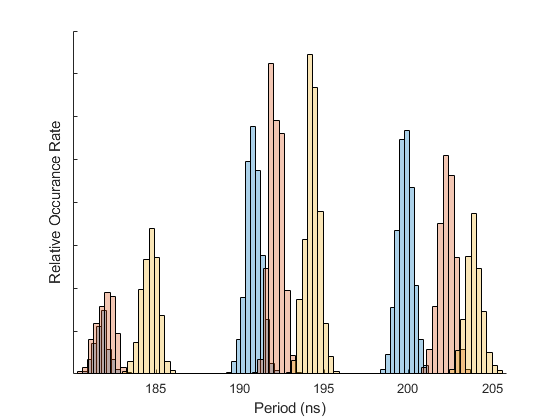
\includegraphics[width=0.5\linewidth]{distrib_ring} }}%
    \subfloat[FPGA Clocked Design.]{{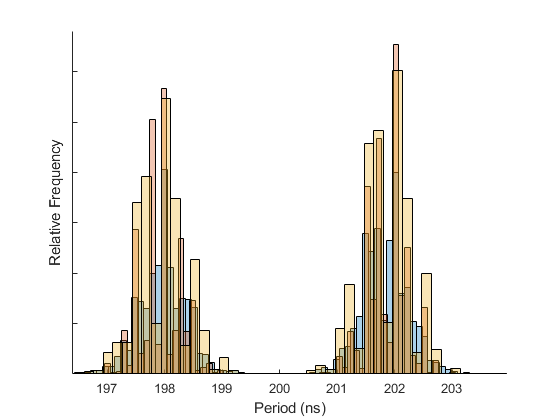
\includegraphics[width=0.5\linewidth]{distrib_pa} }}%
    \caption{Example Distribution of Periods.\label{fig:dists}}    
    \vspace{-0.5cm}
\end{figure}
Figure \ref{fig:dists} paints a picture of the unrealistic nature of the FPGA clocked design in comparison to its inverter based counterpart, each oscillator will have identical intrinsic period steps thus eliminating any jitter that maybe be seen in the system due to misalignment. This effects the suitability of the FPGA clocked designs for the improvement of simulation models, or the examination of how a novel block may impact the behaviour of the network.
\section*{Conclusion}
An FPGA is a suitable environment for the prototyping of ADPLL networks and can fill a number of roles depending on the designer's requirements. However, the designer should bear in mind the platform's limitations, especially when attempting to use a frequency that is not orders of magnitude lower than the maximum clock available from the FPGA's clock manager. Inverter based and FPGA clocked designs, both have a niche in which they are the preferred option, with the clocked design better suiting replication of an existing design at scaled-down frequencies and the inverter based designs better in the modelling and analysis of ADPLL network behaviour.

\bibliographystyle{IEEEtran}
\bibliography{conf} 

\end{document}
%It is apparent that the combination of the inverter chain DCO and the FPGA clocked phase detector is an ill advised choice, with the system's jitter being an order of magnitude worse than the design using inverter delay based detector. In order to obtain measurements for this combination, due to the poor performance, a four times divider was inserted into the feedback path and the comparison made between this divided output and a reference signal at 1.25 MHz, and hence the presence of jitter greater than the period of 200 ns. In this system, the FPGA clock is at 258 MHz, the maximum possible to satisfy timing requirements, thus giving a detection resolution of 3.875 nanoseconds. This is significantly greater than the 1.2 nanosecond period step of the oscillator, requiring an increase in the loop filter gains when compared to the first combination in the table. The problems of relatively inaccurate detection and increased gains combine to produce a system that is only able to achieve poor locking performance. In case three then the detector's resolution improves to 0.6 nanoseconds and produces relatively good system performance. This combination does not perform as well as that of case one, but that is attributable to the unrealistic nature of the FPGA clocked design. Both case one and three work well, delivering a level of jitter that is both low yet allows an indication of how impactful variations in architecture or control parameters are to be seen visually on an oscilloscope with appropriate persistence.\\


%From the table it is apparent that the combination of the inverter chain DCO and the FPGA clock driven phase detector is an ill-advised choice, as the jitter present in the system is several orders of magnitude worse than either other situation. 
%This is 3.5 times greater than the period resolution of approximately 1.2 nano second period resolution of the oscillator, and requires the gains of the PI filter to be increased fourfold in order to respond appropriately to the error detected. The 
%Both other combinations work well however, delivering a level of jitter that is both low yet allows an indication of how impactful variations in architecture or control parameters are to be seen visually on an oscilloscope.\\

